\graphicspath{{Chapitre_6/Images/}}
\chapter{Model overview}\label{C6}
%%%%%%%%%%%%%%%%%%%%%%%%%%%%%%%%%%%
%%%%%                         %%%%%
%%%%% Introduction chapitre 5 %%%%%
%%%%%                         %%%%%
%%%%%%%%%%%%%%%%%%%%%%%%%%%%%%%%%%%
\quad\, In the chapter \ref{C5}, the Brayton cycle has been introduced by presenting two configurations. Also, it has been mentioned that many other configurations (illustrated in the annex \ref{annex:Brayton_variant}) exists to cover a large panel of applications. 

This chapter will be devoted to the description of the  Brayton cycle model. This model, will only consider steady state operations. Thus, transient effects like acceleration of the turbomachines or the heating up of the heat-exchangers will not be taken into consideration.
 

\section{Python language}
%%%%%%%%%%%%%%%%%%%%%%%%%%%%%%%%%%%
%%%%%                         %%%%%
%%%%%  <<Python language>>    %%%%%
%%%%%                         %%%%%
%%%%%%%%%%%%%%%%%%%%%%%%%%%%%%%%%%%
\quad\, Python is a computing language that was created by Guido van Rossum at the Centrum Wiskunde \& Informatica (CWI - \url{https://www.cwi.nl}) in the early 1990s. Starting 1995, G. van Rossum continued to work on Python at the Corporation for National Research Initiatives (CNRI - \url{https://www.cnri.reston.va.us/}). Since the very first release, the language was open source. This means that the source code was accessible to anyone. 

From this time, Python progressively gained in popularity, and the community participating to the development of the software didn't stop to grow. Today, this language is used by many companies and for many types of applications. Indeed, this programming language is used for website creation, machine learning, automation, etc. 

Since Python is an open source language, it lives thanks to its community which creates and shares libraries. Indeed, what have already been implemented in the past can be freely used by the other users. Moreover, new users can easily start developing under Python thanks to huge amount of guide and documentation to starting learning about the Python language.

Also, Python is a programming language that allows the object oriented programming. This paradigm consists in the definition of blocks of code (called objects) which are able to interact together through relations, defined in order to solve a given problem. This allows to create computer code that can evolve through the times. 

\section{Model structure}
%%%%%%%%%%%%%%%%%%%%%%%%%%%%%%%%%%%
%%%%%                         %%%%%
%%%%% <<Structure of the>>    %%%%%
%%%%%      <<model>>          %%%%%
%%%%%                         %%%%%
%%%%%%%%%%%%%%%%%%%%%%%%%%%%%%%%%%%
\quad\, the previous section shows that Python was a great language due to its huge community and the ability to do oriented object programming. Combined with the fact that Python is free and open source, it has been chosen to program the model developed during this master thesis under the Python language.

The focus of this section is the description of the structure of the computer code itself. As it can be expect from what have been previously said, the program will be composed of multiple blocks that will interact together.

\subsection{Inputs}
\quad\, To start the program, the user has to provide an input file that will contain the required data for the program. The input file is structured as a dictionary\footnote{see \url{https://www.w3schools.com/python/python_dictionaries.asp} for further information} and is composed of three main fields. A template of an input file for the gas turbine configuration is given in the annex \ref{annex:Input_file}.

The first field named "Type" says to the computer code which configuration of the Brayton cycle has to be assess. The possible configurations are listed in Table \ref{tab:C5_inputconfig}.

\begin{longtable}[c]{ll}
\caption{Program input - "Type" field}
\label{tab:C5_inputconfig}\\
\toprule
\textbf{Type - Acronym} & \textbf{Type - Name}                   \\* \midrule
\endfirsthead
%
\endhead
%
\bottomrule
\endfoot
%
\endlastfoot
%
GT                           & Gas Turbine                                 \\
RGT                          & Regenerative Gas Turbine                    \\
IRGT                         & Intercooler-Regenerative Gas Turbine        \\
RHGT                         & Regenerative-Reheat Gas Turbine             \\
IHGT                         & Intercooler-Reheat Gas Turbine              \\
IRHGT                        & Intercooler-Regenerative-Reheat Gas Turbine \\
EFGT                         & Externally-Fired Gas Turbine                \\* \bottomrule
\end{longtable}

These different configurations are described in the annex \ref{annex:Brayton_variant}. 

The second field list all the input data required to initialized the model. The number of variables to be specified at the start of the program depends on the selected configuration. For instance, considering the gas turbine (GT), the inputs required are listed in Table \ref{tab:C5_inputGT}.
\begin{longtable}[c]{ll|ll}
\caption{Input - gas turbine (GT)}
\label{tab:C5_inputGT}\\
\toprule
\textbf{Inputs - Name}                                                                          & \textbf{Inputs - Abbreviation} & \textbf{Inputs - Name}                                                                                          & \textbf{Inputs - Abbreviation} \\* \midrule
\endfirsthead
%
\endhead
%
\bottomrule
\endfoot
%
\endlastfoot
%
\begin{tabular}[c]{@{}l@{}}Reference \\ temperature (°C)\end{tabular}                  & $T_{ref}$             & \begin{tabular}[c]{@{}l@{}}Combustion chamber \\ efficiency (\%)\end{tabular}                          & $\eta_{cc}$           \\
\begin{tabular}[c]{@{}l@{}}Ambient \\ temperature (°C)\end{tabular}                    & $T_{amb}$             & \begin{tabular}[c]{@{}l@{}}Shaft mechanical \\ efficiency (\%)\end{tabular}                            & $\eta_{shaft}$        \\
\begin{tabular}[c]{@{}l@{}}Fuel \\ temperature (°C)\end{tabular}                       & $T_{fuel}$            & \begin{tabular}[c]{@{}l@{}}Generator \\ efficiency (\%)\end{tabular}                                   & $\eta_{gen}$          \\
\begin{tabular}[c]{@{}l@{}}Combustion chamber \\ exhaust temperature (°C)\end{tabular} & $T_{cc,ex}$           & \begin{tabular}[c]{@{}l@{}}Compressor isentropic \\ efficiency (\%)\end{tabular}                       & $\eta_{comp}$         \\
\begin{tabular}[c]{@{}l@{}}Reference \\ pressure (Pa)\end{tabular}                     & $p_{ref}$             & \begin{tabular}[c]{@{}l@{}}Turbine isentropic \\ efficiency (\%)\end{tabular}                          & $\eta_{t}$            \\
\begin{tabular}[c]{@{}l@{}}Ambient \\ pressure (Pa)\end{tabular}                       & $p_{amb}$             & \begin{tabular}[c]{@{}l@{}}Compressor \\ pressure ratio (-)\end{tabular}                               & $P_{comp,ratio}$      \\
\begin{tabular}[c]{@{}l@{}}Duct \\ pressure drop (\%)\end{tabular}                     & $Dp_{duct}$           & \begin{tabular}[c]{@{}l@{}}Air mass \\ flow rate (kg/s)\end{tabular}                                   & $\dot{m}_{air}$       \\
\begin{tabular}[c]{@{}l@{}}Combustion chamber \\ pressure drop (\%)\end{tabular}       & $Dp_{cc}$             & \begin{tabular}[c]{@{}l@{}}Nominal mass \\ flow rate (kg/s)\end{tabular}                               & $\dot{m}_{nom}$       \\
Chimney suction (Pa)                                                                   & $Dp_{chimney}$        & Air factor (-)                                                                                         & $\lambda$             \\
Fuel composition (\%)                                                                  & $Fuel_{char}$         & \begin{tabular}[c]{@{}l@{}}{\color{PineGreen}{Compressor}} \\ {\color{PineGreen}{performance map}} (.xls/.xlsx)\end{tabular} & $Comp_{excel}$        \\
Air composition (\%)                                                                   & $Air_{char}$          & \begin{tabular}[c]{@{}l@{}}{\color{PineGreen}{Turbine}} \\ {\color{PineGreen}{performance map}} (.xls/.xlsx)\end{tabular}    & $Turb_{excel}$        \\
{\color{Gray} Rotational speed} (rpm)                                                  & $N$                   &                                                                                                        &                       \\* \bottomrule
\end{longtable}

The last field named "Selection" is composed of two boolean variables. The first one gives the choice to add a water heat exchanger between the \textit{end} of the cycle and the exhaust. When this variable, named "WHX", is set to \textit{true}, the following inputs as to be added.

\begin{itemize}
\setstretch{1}
\item Water inlet temperature (\degree C): $T_{whx,su,w}$
\item Water outlet temperature (\degree C): $T_{whx,ex,w}$
\item Water inlet pressure (Pa): $p_{whx,su,w}$
\end{itemize}

"MAP" is the second variable. It used to choose whether or not the performance map for the turbomachines (defined as in chapter \ref{C4}). If the variable is set to \textit{true}, the {\color{Gray} gray} field in Table \ref{tab:C4_inputGT} is at least required. Then, depending on the validity of the {\color{PineGreen} pinegreen} fields, the compressor and/or the turbine map(s) will be used in the code. 

When a valid compressor map is given, the variables $\eta_{comp}$ and $P_{comp,ratio}$ are not required to be filled. Indeed, as seen in chapter \ref{C4}, the knowledge of two independent operating variables are sufficient to derived the other variables. In particular, the rotational speed $N$, the air mass flow rate and the inlet state of the compressor are known. Thus, using the relation (\ref{eq:C4_mc}) to obtain the corrected mass flow rate $\dot{m}_{c,comp}$ through the compressor, the compression ratio and the compressor efficiency can be derived.  

Similarly, if a valid turbine map is provided in the inputs, the turbine isentropic efficiency $\eta_{t}$ and the combustion chamber exhaust temperature $T_{cc,ex}$ specified in the inputs will not be used. From the knowledge of the compression ratio, the expansion ratio $P_{turb,ratio}$ can be obtained by computing the pressure drops within the cycle. Then, the efficiency and the corrected mass flow rate $\dot{m}_{c,turb}$ can be derived since two independent variables are known.

The knowledge of both the corrected and \textit{not} corrected mass flow rate through the turbine are sufficient to compute the turbine inlet temperature (TIT). Indeed, the relation (\ref{eq:C4_mc}) from chapter \ref{C4} can be rewritten as followed

\begin{equation}
    \setstretch{1}
TIT =T_{ref}\cdot \left(\frac{\dot{m}_c}{\dot{m}}\cdot\frac{p}{p_{ref}}\right)
\end{equation} 

which allows the computation of the turbine inlet temperature.
\newpage
\subsection{Flow chart of the model}
\quad\,  The previous section detailed the the structure of the input file to be provided at the start of the program. Once provided, the program will first read the "Type" field to select the desired configuration. If the configuration is contained in the database of the program, the associated model will be created.
\begin{wrapfigure}{l}{0.42\linewidth}
\centering
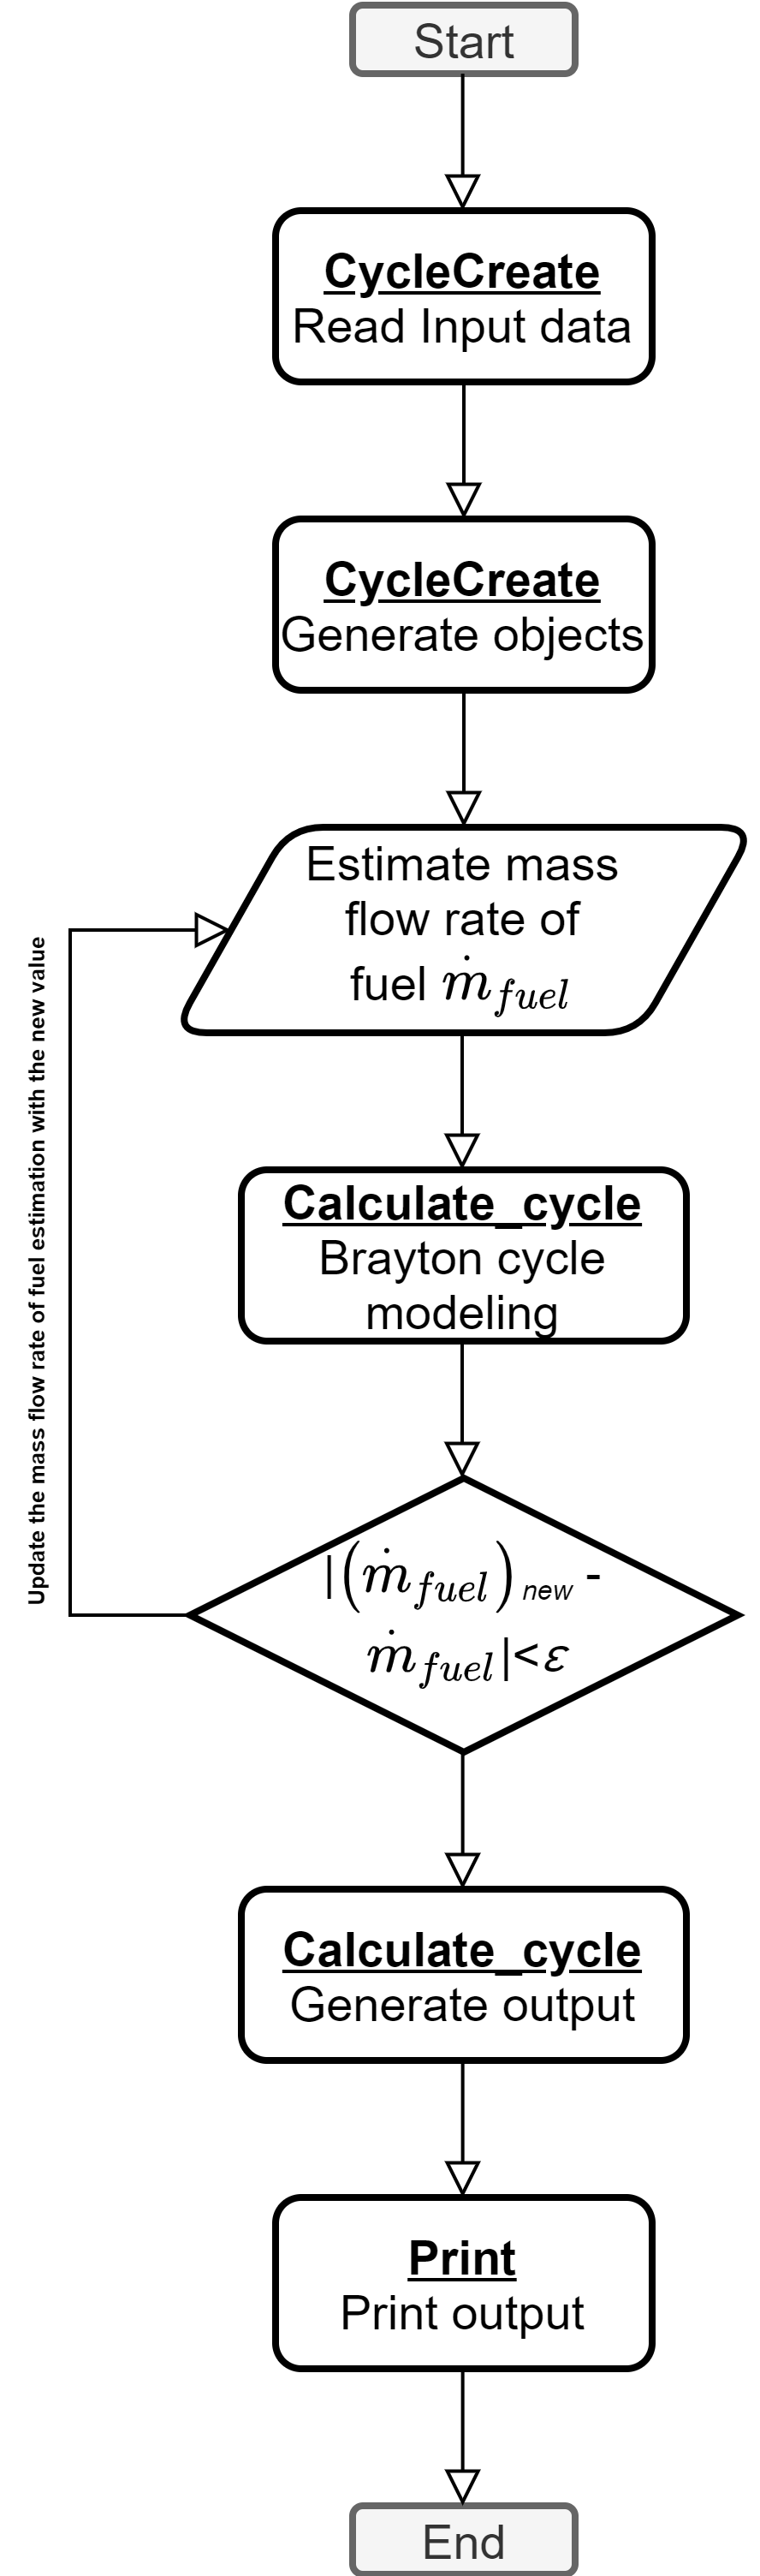
\includegraphics{Flow_chart.png}
\caption{Flow chart of the Brayton cycle model}
\label{fig:C6_flowchart}
\end{wrapfigure}
The second step consists in the reading and storage of the input data from the input file. Then, a restructuring of the input is performed to be understood by the model. This extraction of data is performed regarding to value of the variables within the field "Selection".

When all the required inputs are loaded, the program starts the model. To initiate the assessment of the performance of the selected cycle, a initial guess on the mass flow rate of fuel $\dot{m}_{fuel}$ is realized. Then, the model \textit{travels} along the cycle by calling the objects associated to the real components. 
After having gone through the combustion chamber(s), the mass flow rate of fuel is re-evaluated to update the initial guess. If the change is smaller than $\varepsilon$, the model escapes the loop. Otherwise, new passages are performed until no noticeable change of the mass flow rate value.
   
Finally, outputs are generated based on the assessed cycle. Among these, the temperature, pressure, enthalpy, and density at each state of the cycle are specified. The fuel mass flow rate is also provided to the user along with the thermal efficiency of the cycle and the power consumed and produced. 

This structure is followed for every selected configurations. The flow chart on Figure \ref{fig:C6_flowchart} graphically illustrates the structure of the model from the reading of the inputs to the generation of the outputs.\clearpage

As it has been presented, the main structure of the program is relatively linear without many branches. This linear scheme allows a rapid comprehension of how the program works from the outside. However, when considering the calls of the objects in the ''Calculate\_cycle'' function, the structure becomes more complex. 

Thus, this main function relies on objects to live within the program.  Among these objects, two categories, namely the \textbf{static} and \textbf{non-static} object, can be defined.

The first category called \textbf{static} objects are the objects associated to the thermodynamic components (compressor, turbine,etc...). These objects are called statics because each of the components will not change of position in the cycle once the latter is defined. \\

Then, there are the objects representing the fluids involved in cycle. These \textbf{non static} objects will live the thermodynamic cycle by going through the different components.

For a Brayton cycle, the modeled fluids are typically air, fuel, exhaust gas, and sometimes water (if there is any water heat exchanger). This explicit definition for each of these fluids is useful. Indeed, it allows to create a more flexible model since the modification of one fluid composition has only to be performed while defining the associated object. 

The next chapter will present the implementation method of each thermodynamic components. For each of those, the functions involved will be defined and explained. Also, some links with the theoretical notions seen in chapters \ref{C2}, \ref{C3} and \ref{C4} will be created.





 